%-*- coding: UTF-8 -*-
%gougu.tex
% 勾股定理
\documentclass[UTF8]{ctexart} %因为是中文的短文,所以使用ctexart
\usepackage{graphicx}	%插图内容需要用到的graphicx宏包
\usepackage{float}		%float宏包
\usepackage{amsmath}	%数学宏包
\usepackage{geometry}	%设计页面尺寸可以用geometry宏包
\geometry{a6paper,centering,scale=0.8}
						%设定图表所有标题使用悬挂对齐方式(即编号向左突出),
						%整体用小字号,而标题文本使用斜体(对汉字来说就是楷书)。
						%改变图表标题格式可以使用caption 宏包
\usepackage[format=hang,font=small,textfont=it]{caption}
						%增加目录的项目则可以用tocbibind 宏包
						%这里使用nottoc 选项取消了在目录中显示目录本身
\usepackage[nottoc]{tocbibind}
						%利用\newenvironment 命令定义一个新的环境	
\newenvironment{myquote}	
	{\begin{quote}\kaishu\zihao{-5}}
	{\end{quote}}	
						%可以用\newcommand 命令定义一个新的命令\degree	
\newcommand{\degree}{^\circ}					
						
\title{\heiti 杂谈勾股定理}
\author{\kaishu 张三}
\date{\today}

\bibliographystyle{plain}	%声明参考文献的格式
\newtheorem{thm}{定理}



\begin{document}	%之前部分用于对文档进行设置
					%注意要生出目录至少编译两次
\maketitle	%输出论文标题,使结果显现出来
\begin{abstract}	%摘要
	这是一篇关于勾股定理的小短文。
\end{abstract}	
\tableofcontents	%输出目录

\section{勾股定理在古代}
西方称勾股定理为毕达哥拉斯定理,将勾股定理的发现归功于公元前 6 世纪的
毕达哥拉斯学派 \cite{Kline}。该学派得到了一个法则,可以求出可排成直角三角形三边的三
元数组。毕达哥拉斯学派没有书面著作,该定理的严格表述和证明则见于欧几里
德\footnote{欧几里德,约公元前330--275 年。}《几何原本》的命题 47:
“直角三角形斜边上的正方形等于两直角边上的两个正方形之和。”证明是用面积做的。

我国《周髀算经》载商高(约公元前 12 世纪)答周公问:
\begin{myquote}
	 勾广三,股修四,径隅五。
\end{myquote}
又载陈子(约公元前7--6 世纪)答荣方问:
\begin{myquote}
	 若求邪至日者,以日下为勾,日高为股,勾股各自乘,并而开方除之,得邪至日。
\end{myquote}
都较古希腊更早。后者已经明确道出勾股定理的一般形式。图1是我国古代对勾股定理的一种证明\cite{quanjing}。
%[ht],表示浮动体可以出现在环境周围的文本所在处
%(here)和一页的顶部(top)
\begin{figure}[ht]
	\centering
	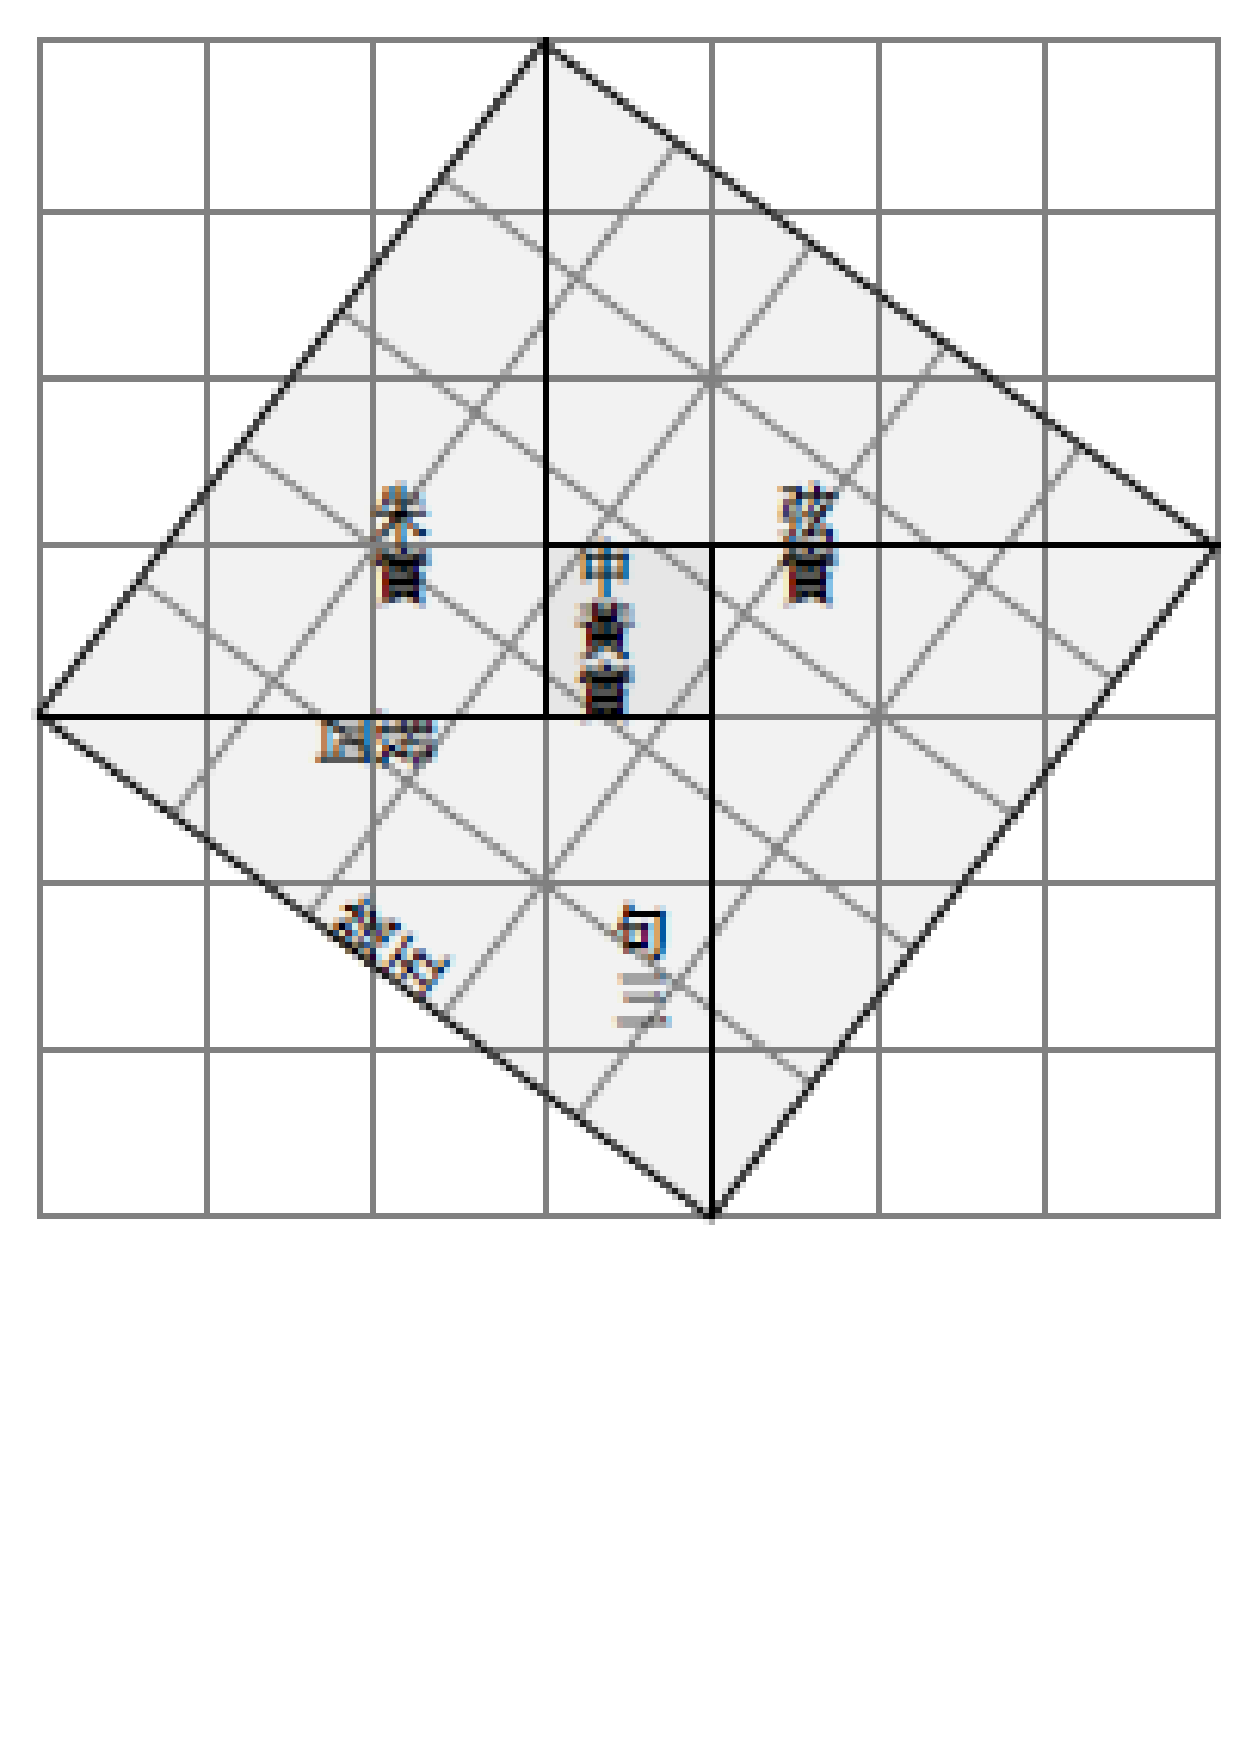
\includegraphics[scale=0.15]{xiantu.pdf}	%要在导言区引用graphicx宏包
	\caption{宋赵爽在《周髀算经》注中作的弦图(仿制),该图给出了勾股定理的一个极具对称美的证明}
	\label{fig:xiantu}
\end{figure}

\section{勾股定理在近代形式}
勾股定理可以用现代语言表述如下:
\begin{thm}[勾股定理]
	直角三角形斜边的平方等于两腰的平方和。
	
	可以用符号语言表述为:设直角三角形ABC,其中$\angle C = 90\degree$,则有
\begin{equation}\label{eq:gougu}
AB^2 = BC^2 + AC^2.
\end{equation}
	
满足式\eqref{eq:gougu}的整数称为\emph{勾股数}。第1节所说毕达哥拉斯学派得到的三元数组就是勾股数。下表列
出一些较小的勾股数:
\begin{table}[H]	%这段代码要在导言区引用float宏包的这种不浮动的图表环境
\begin{tabular}{|rrr|}	%右对齐
\hline
直角边 $a$ & 直角边 $b$ & 斜边 $c$	\\
\hline
3 &	4 &	5\\
5 &	12 & 13\\
\hline	
\end{tabular}%
\qquad	%产生长为2em的空白
($a^2+b^2=c^2$)
\end{table}
\end{thm}

\nocite{Shiye}	%在列表显示并不直接引用的文献
\bibliography{math}	%打印出参考文献列表

\end{document}